\section{Results}

Implementation of the our approach is provided in the \R\ package
\href{https://dajmcdon.github.io/rtestim/}{\texttt{rtestim}}. All experiments
are run in \R\ with version 4.3.1 on a MacBook with an Apple M1 Pro chip
and 32GB RAM running under macOS Sonoma 14.0. The \R\ packages used for
simulation and real-data application are versions \texttt{EpiEstim 2.2-4},
\texttt{EpiLPS 1.2.0}, and \texttt{rtestim 0.0.4}. 

\subsection{Simulation settings}

% problem settings
%% Rt
We simulate four scenarios of the time-varying effective reproduction numbers,
intended to mimic different epidemics. The first two scenarios are simple cases
that are rapidly controlled by intervention, where the graphical curves consist
of one discontinuity and two segments. Scenario 1 has constant $\calR_t$ before
and after an intervention, while Scenario 2 grows exponentially, then decays.
The other two scenarios are more complicated, where more waves in the epidemics
are involved. Scenario 3 has four linear segments with three discontinuities,
which reflect the effect of an intervention, resurgence to rapid transmission,
and finally suppression of the epidemic. Scenario 4 involves sinusoidal waves
throughout the epidemic.
% motivation
The first three scenarios and the last scenario are motivated by
\citet{parag2021improved} and \citet{gressani2022epilps} respectively. 
% name the scenarios
We name the four scenarios as \textit{(1) piecewise constant}, \textit{(2) piecewise exponential}, 
\textit{(3) piecewise linear}, and \textit{(4) periodic} lines or curves respectively. 

In all cases, the times of observation are regular, and epidemics are of
length $n=300$. Specifically, in Scenario 1, $\calR_t = 2, 0.8$ before and after
$t=70$. In Scenario 2, $\calR_t$ increases and decreases exponentially with
rates $0.015, 0.005$ pre and post $t=50$. 
In Scenario 3, $\calR_t$ is piecewise linear with four discontinuous segments following 
\begin{align*}
    \calR(x) = & \lr{2.5 - \frac{0.5}{59}\lr{x-1}} \boldsymbol{1}_{[1,60]}(x)
     + \lr{0.8 - \frac{0.2}{49}\lr{x-61}} \boldsymbol{1}_{(60,110]}(x) \\
    & + \lr{1.7 + \frac{0.3}{39}\lr{x-111}} \boldsymbol{1}_{(110,150]}(x)
     + \lr{0.9 - \frac{0.4}{149}\lr{x-151}} \boldsymbol{1}_{(150,300]}(x),
\end{align*}
where $\boldsymbol{1}_{A}(x) = 1$, if $x\in A$, and $\boldsymbol{1}_{A}(x)=0$ otherwise. 
In Scenario 4, $\calR_t$ is realization of the 
continuous, periodic curve generated by the function $$\calR(t) = 0.2 \big(
\lr{\sin(\pi t/12) + 1} + \lr{2 \sin\lr{\pi t / 6} + 2} + \lr{3
\sin(\pi t / 1.2) + 3}\big),$$ evaluated at equally spaced points $t\in [0,10]$. These
settings are illustrated in the left column of \autoref{fig:samples}.


%% other problem settings
We assume that the serial interval follows Gamma distribution with fixed shapes
and scales $(3,3)$, $(2.5,2.5)$, $(3.5,3.5)$ and $(3.5,3.5)$ for Scenarios 1--4
respectively. We consider all epidemics starting from $y_1=2$ cases and
generating until timepoints $t=300$. We compute the expected incidence
$\Lambda_t$ using the renewal equation, and generate the incident samples from
the Poisson distribution $y_t\sim \textrm{Pois}(\Lambda_t)$. To verify the
performance of our model under the violation of this distributional assumption
of incidence, we also generate incident samples using the negative Binomial
distribution with dispersion size 5, i.e., $y_t\sim \textrm{NB}(\Lambda_t,
\textrm{size}=5)$. We generate 50 random samples for each setting of
experiments, resulting in 400 total experiments. An example of each effective
reproduction number scenario with a single corresponding Poisson and negative
Binomial sample incidence sequences is displayed in \autoref{fig:samples}. 

\begin{figure}[hp!]
    \centering
    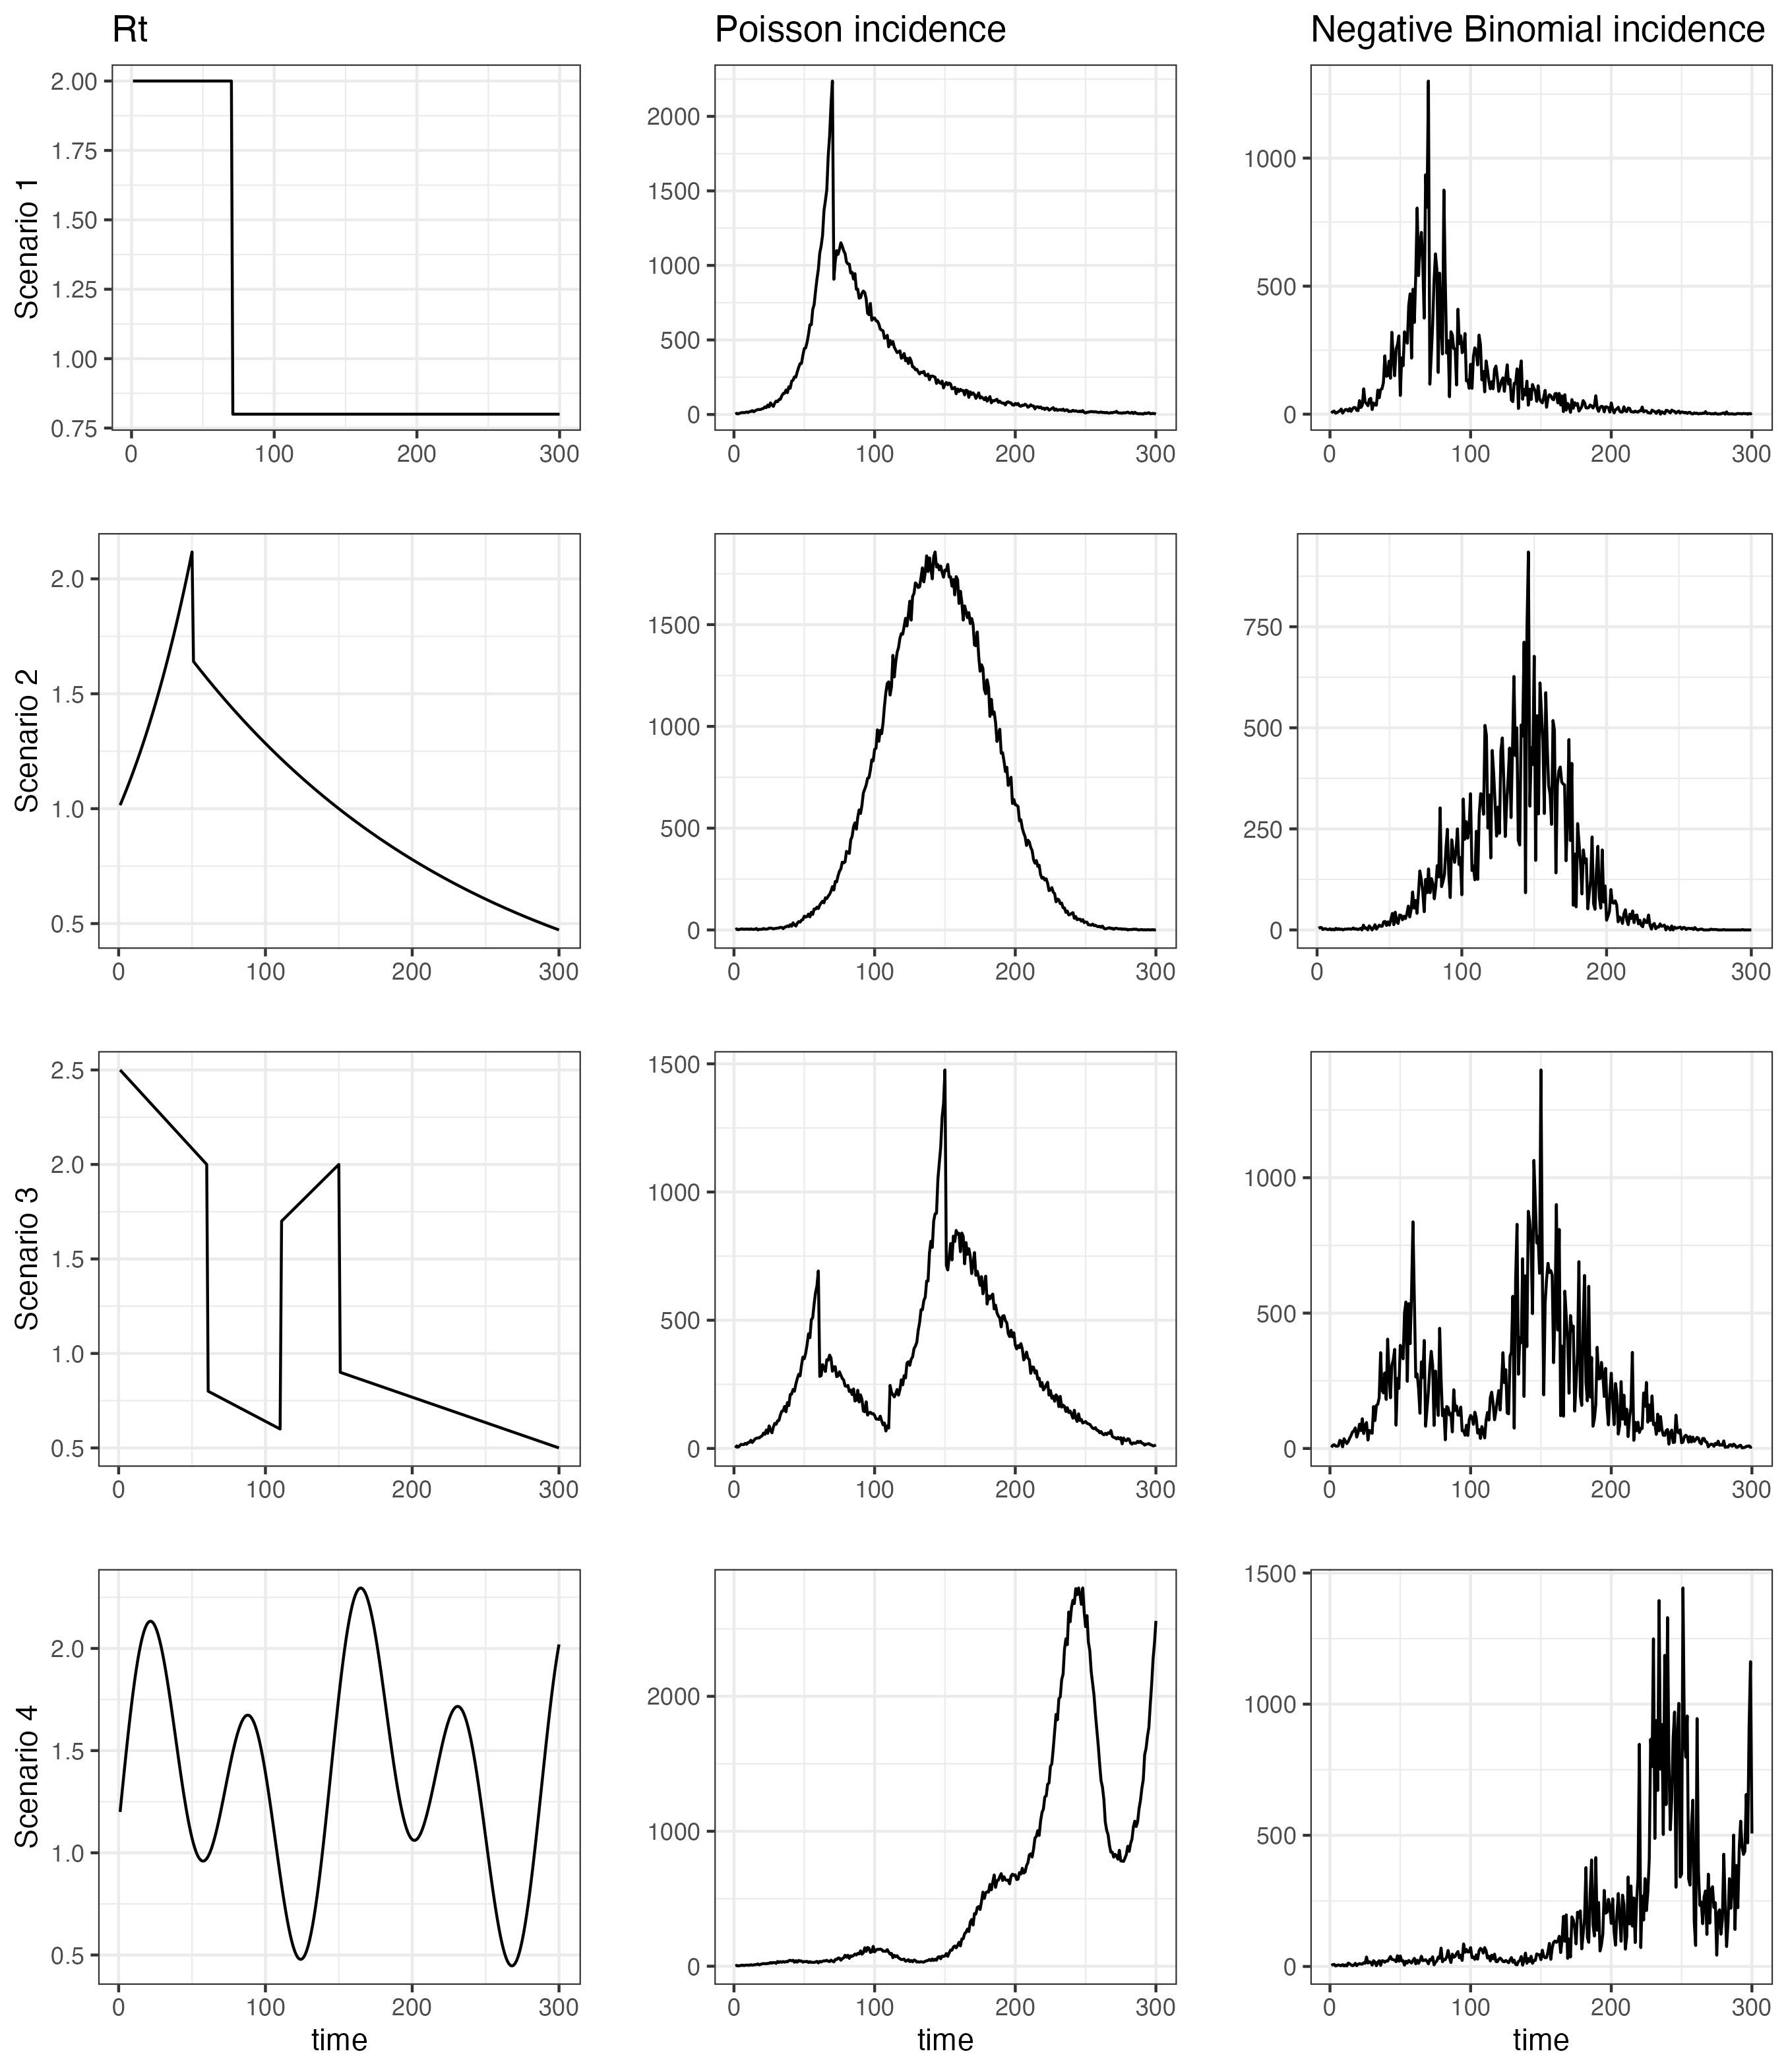
\includegraphics[width=.9\textwidth]{fig/plot_samples.png}
    \caption{The effective reproduction numbers (left column) and corresponding
    sample incident cases drawn from a  Poisson (middle column) or negative
    Binomial (right column) distribution. The rows correspond to the four
    $\calR_t$ settings.} 
    \label{fig:samples}
\end{figure}

% algorithm settings
%% competitors and their settings
We compare \RtEstim\ to \EpiEstim\ and \EpiLPS. Unfortunately,
\texttt{EpiFilter} frequently fails to converge due to the large case counts in
many simulations. \EpiEstim\ estimates the posterior distribution of effective
reproduction numbers given a Gamma prior and Poisson distributed incidence. It
estimates the reproduction number over a sliding window, assuming the
reproduction number is constant during the specific time window. A longer
sliding window averages out more fluctuations, leading to smoother estimates,
whereas, a shorter sliding window is more responsive to sudden spikes or
declines. We tried the default, a weekly sliding window, as well as a monthly
window. However, since neither considerably outperforms the other across all
scenarios, we defer the monthly case to the Appendix. \EpiLPS\ is another
Bayesian approach that estimates P-splines coupled with Laplace approximations
of the conditional posterior based on the negative Binomial likelihood. For
\RtEstim\ on the four scenarios respectively, we estimate (1) piecewise constant
$k=0$, (2) piecewise linear \& cubic $k=1,3$, (3) piecewise linear $k=1$ and (4)
piecewise cubic polynomials $k=3$. In each case, we examine a grid of 50
$\lambda$ values, selecting the best using 10-fold cross validation. For all models and
problems, we use the serial interval distribution used to create the data. 

% KL for exponential family: 
To measure estimation accuracy, we compare $\widehat{\calR}$ to $\calR$ using
the Kullback-Leibler (KL) divergence: a standard metric that measures the
distance between two probability distributions. Since $\calR_t$ can be regarded
as the expectation of Poisson distribution, we use the KL divergence for
Poisson distributions (averaged across all coordinates) to measure the accuracy
of the $\calR_t$ estimates 
$$D_{KL}(\calR \parallel \widehat{\calR}) = \sum_{t=1}^n w_t \lr{\calR_t \log\left(\frac{\calR_t}
{\widehat{\calR}_t}\right) + \widehat{\calR}_t - {\calR}_t},$$ 
where $\calR = \left\{ \calR_t \right\}_{t=1}^n$ and 
$w_t = \eta_t / \sum_t \eta_t$ is the rescaled total infectiousness.
To fairly compare across methods, we drop the estimates during the first
week because estimates from \EpiEstim\ do not begin until $t=8$ (using a weekly
window). KL divergence is more appropriate for measuring accuracy because it
connects directly to the Poisson likelihood used to generate the data, whereas
standard measures like the mean-squared error correspond to Gaussian data. This
has the effect of increasing the relative cost of mistakes when $\Lambda_t$ is small.
%For negative Binomial cases, we use KL divergence to measure the distances between negative Binomial distributions given the %dispersion rate $\phi$, i.e., 
%\begin{align*}
%    \frac{1}{n} D^{\ast}_{KL}\lr{\hat{\calR}|| \calR} = \frac{1}{n}\sum_{t=1}^n \hat{\calR}_t \log \left(\frac{\hat{\calR}_t}%{\calR_t}\right) + \lr{\hat{\calR}_t + \phi} \log\lr{\frac{\hat{\calR}_t + \phi}{\calR_t + \phi}}. 
%\end{align*}
%\attn{I think this is a good try, but I don't like the resulting figures. Do you? In it's current state, I think this has more costs %(takes more explanation) than benefits (prettier figures). I say we delete the next paragraph and go back to the KL directly (no %baseline).}
%For a better interpretation of model performance, we introduce a baseline performance of
%$\calR^{\ast}$, which is the sliding average of past true $\calR$. We take 
%the sliding window to be a week, which is similar as the setting of the estimators 
%used in the experiments. Specifically, $\calR^{\ast}_t$ at time $t>7$ is set to be 
%the average of $\calR^{\ast}_{t-7},\cdots,\calR^{\ast}_{t-1}$. 
%The baseline $\calR^{\ast}_t$ performance represents the ``close-to-best'' performance 
%that we can achieve given the knowledge of $\calR$. 
%All KL divergences between $\widehat{\calR}$ and $\calR$ are divided by the 
%corresponding baseline, i.e., KL divergence between $\calR^{\ast}_t$ and $\calR$, 
%to conduct the KL ratio $r = \frac{D_{KL}(\calR \parallel \widehat{\calR})}{D_{KL}(\calR \parallel \calR^{\ast})}$. 
%If $r<1$, $\widehat{\calR}$ outperforms the baseline; the larger the ratio is, 
%the worse the performance of $\widehat{\calR}$ is. 
Other details of the experimental settings are deferred to the Appendix. 


\subsection{Simulation results}

\RtEstim\ overall outperforms \EpiEstim\ and \EpiLPS\ in the experimental study.
\autoref{fig:kl-res} visualizes the KL divergence across the three models. Under
both Poisson and negative Binomial distributions, \RtEstim\ is easily the most
accurate across Scenarios 1 and 3: the median of KL divergence is much lower
and the boxes frequently fail to overlap indicating a better performance than
the other two methods across all 50 simulations. 
The advantage is less for the
negative Binomial case compared to the Poisson case, but still obvious. 
% 
\RtEstim\ and \EpiLPS\ have similar performance in Scenarios 2 and 4. 
For the Poisson case, \RtEstim\ and \EpiLPS\ both have very small KL scores, which are
very close to 0. In Scenario 4, \RtEstim\ is slightly better for Poisson and \EpiLPS\ 
is better for negative Binomial, but the boxes largely overlap each other. 
\EpiLPS\ has a slightly lower median and a smaller IQR in Scenario 2 for the negative Binomial case. 
The two degrees of \RtEstim\ used for Scenario 2 perform very close to each other 
for both distributions, which implies a low risk of model misspecification. 
% 
We will examine a single
realization of each experiment to investigate these global conclusions in more
detail.

\begin{figure}[htb]
    \centering
    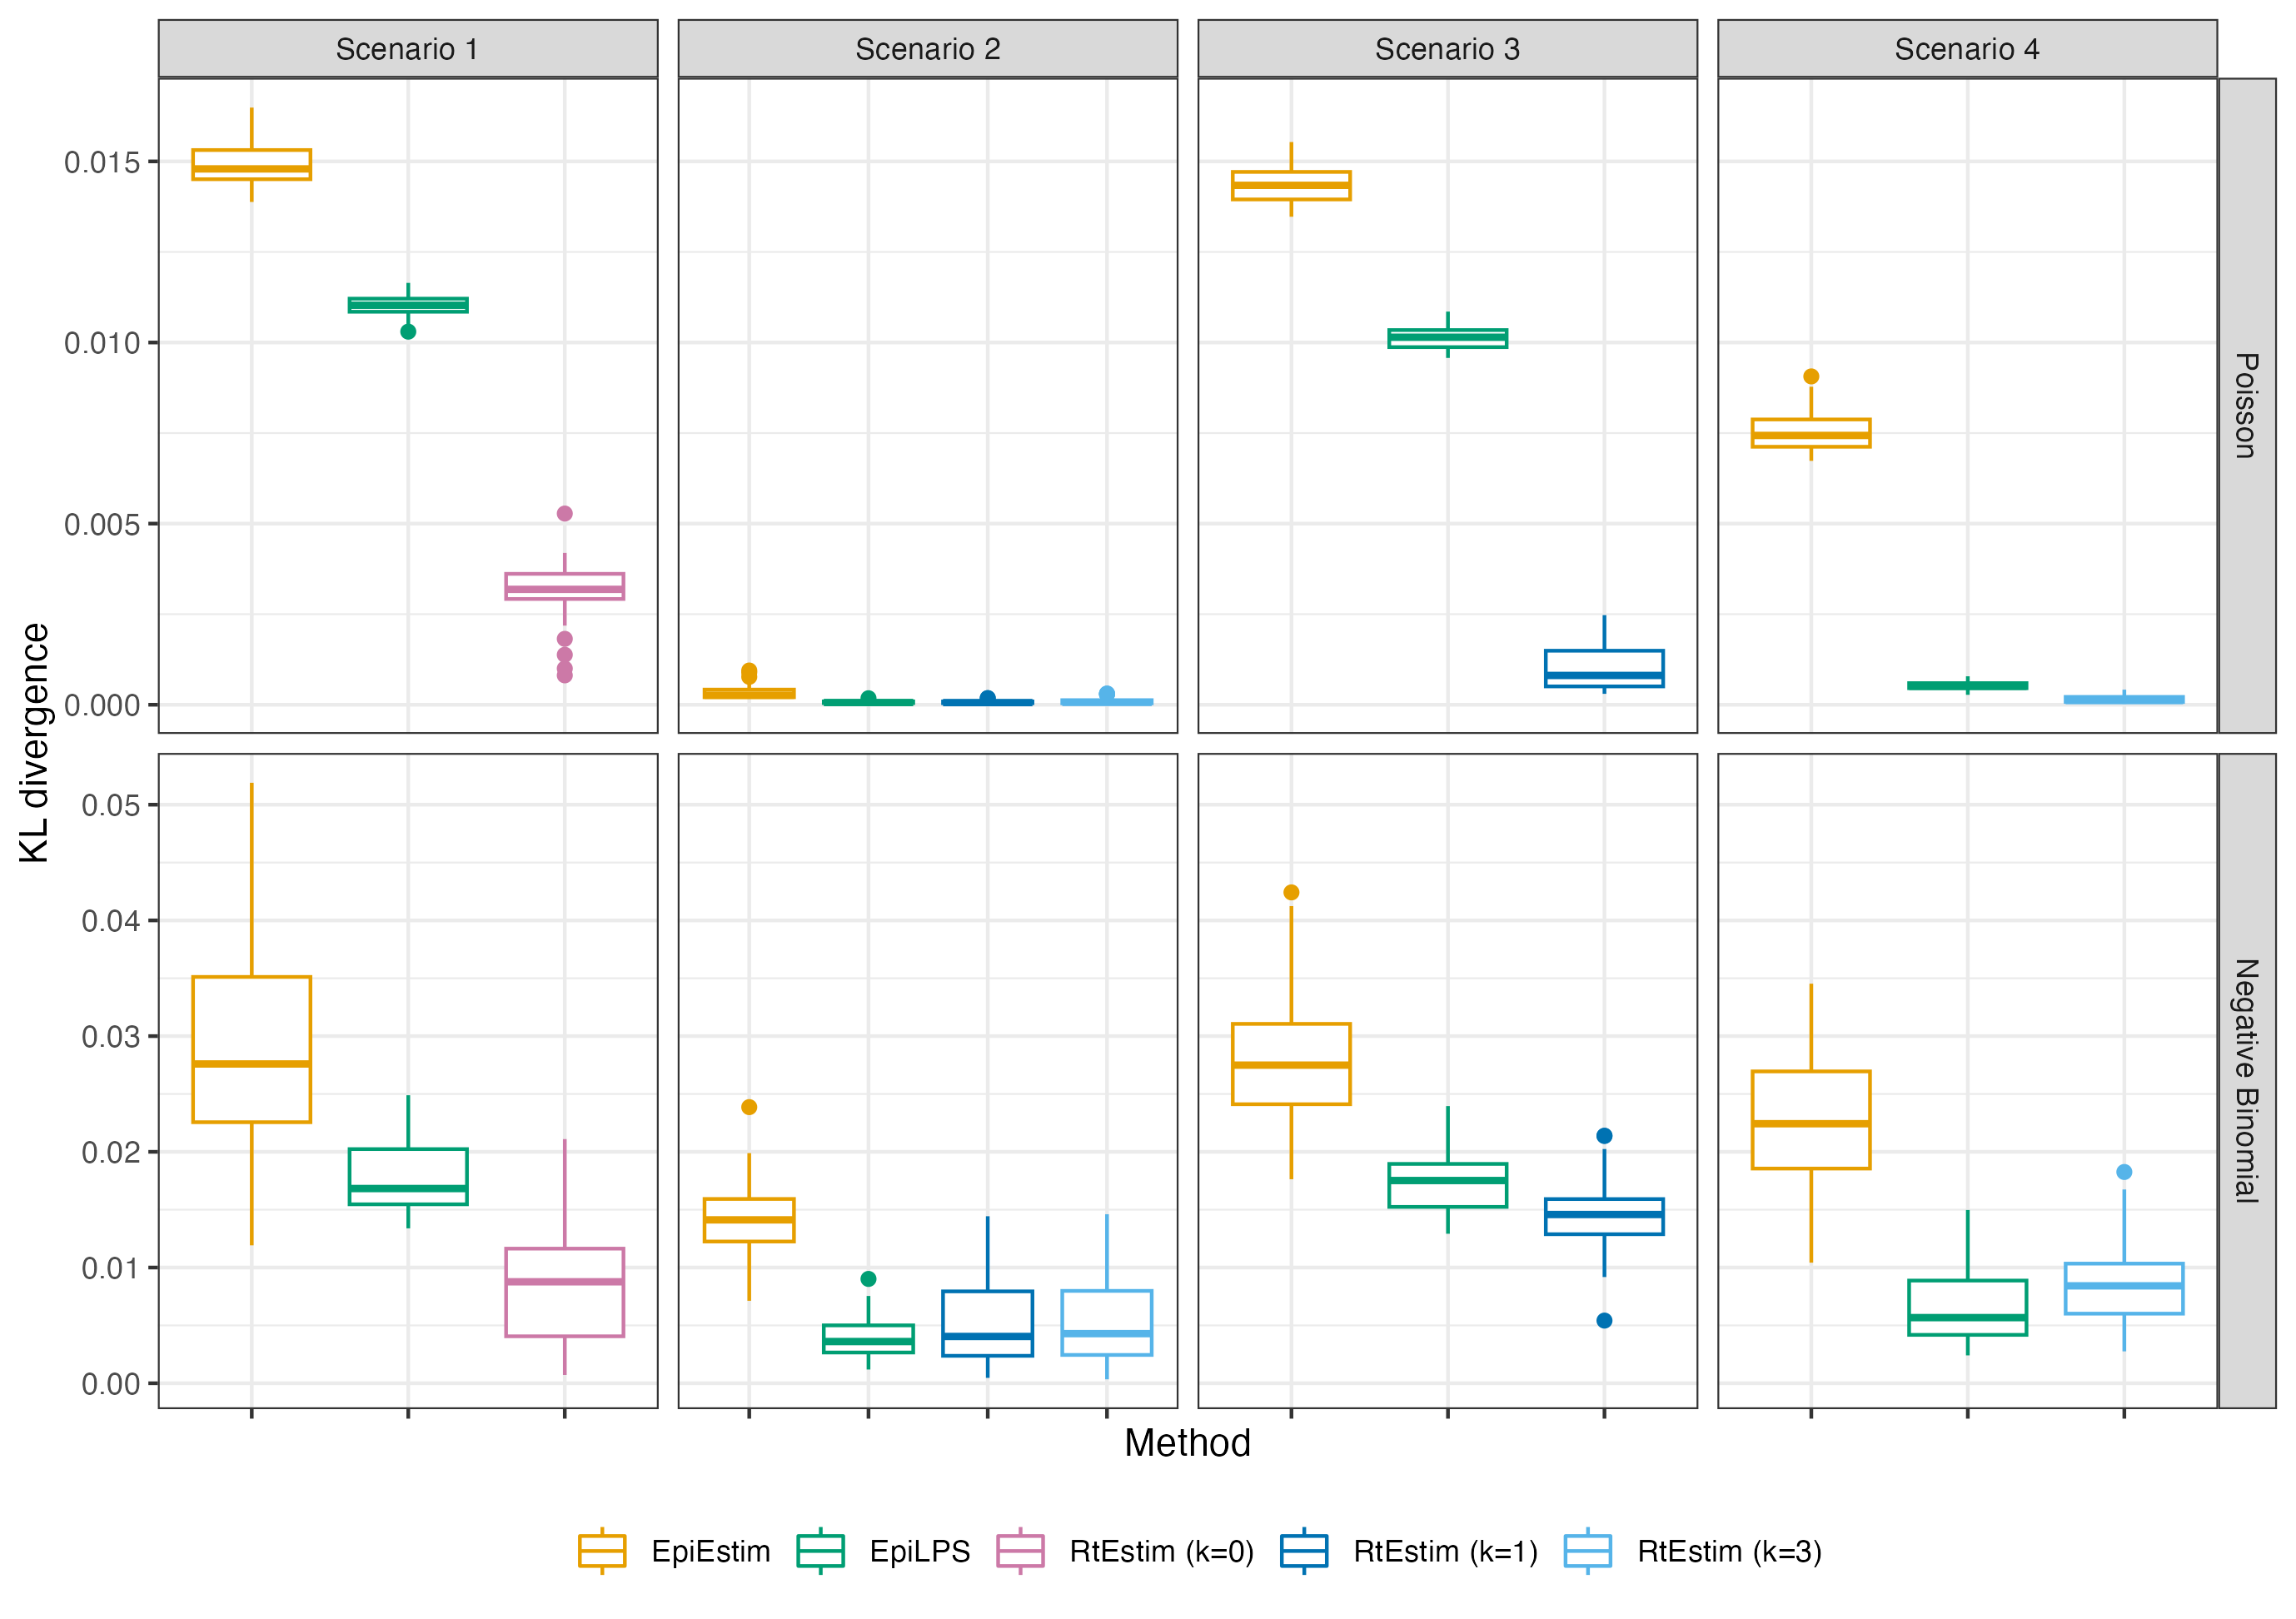
\includegraphics[width=.99\textwidth]{fig/KL_no_outlier.png}
    \caption{Boxplot of KL divergence between the estimated 
    $\hat{\calR}_t$ and the true $\calR_t$ across 50 random samples for 
    each approach given Poisson incidence \textit{(in top panels)} and negative 
    Binomial incidence \textit{(in bottom panels)} respectively.  
    Outliers are excluded. Full visualization is deferred to the Appendix.} 
    \label{fig:kl-res}
\end{figure}


% experiment results
\autoref{fig:pois-est} shows 1 realization for the estimated reproduction
numbers under the Poisson generative model for all 4 scenarios. Compared to
\EpiEstim\ and \EpiLPS, which have rather severe difficulties at the beginning
of the time series, \RtEstim\ estimates are more accurate --- they nearly overlap
with the true values --- without suffering from the edge problem. 
Scenario 2 presents an easy problem in terms of accurate estimation for all methods, 
except at the change point occurring at the end of the exponential growth. 
Although the truth is likely best represented with a piecewise cubic curve, the actual
curvature is so gentle that linear estimation ($k=1$) appears potentially
reasonable. We, therefore, fit piecewise linear and cubic $\hat{\calR}_t$ curves
using \RtEstim\ for Scenario 2 to evaluate model misspecification. 
However, \RtEstim\ with both degrees have difficulty recovering the acute rise 
in the growth phase. Due to this, \RtEstim\ has difficulty in convergence and 
can require more than $10^7$ iterates for all models across the $\lambda$ sequence 
and $10$-fold CV to converge in a couple of simulation samples. 
An explanation of such failure is that the model imposes discontinuity at the
changepoint, which hinders the estimates from fitting the two discontinuous
phases. Scenario 1 is the simplest case with only one knot and two constant
segments. Besides the edge problem, \EpiEstim\ and \EpiLPS\ produce ``smooth''
estimated curves that are continuous at the changepoint, which results in
large mistakes in that neighbourhood. Since the piecewise constant 
\RtEstim\ estimator does not force any smoothness in $\calR_t$, it easily 
captures the sharp change. 

\begin{figure}[tb]
    \centering
    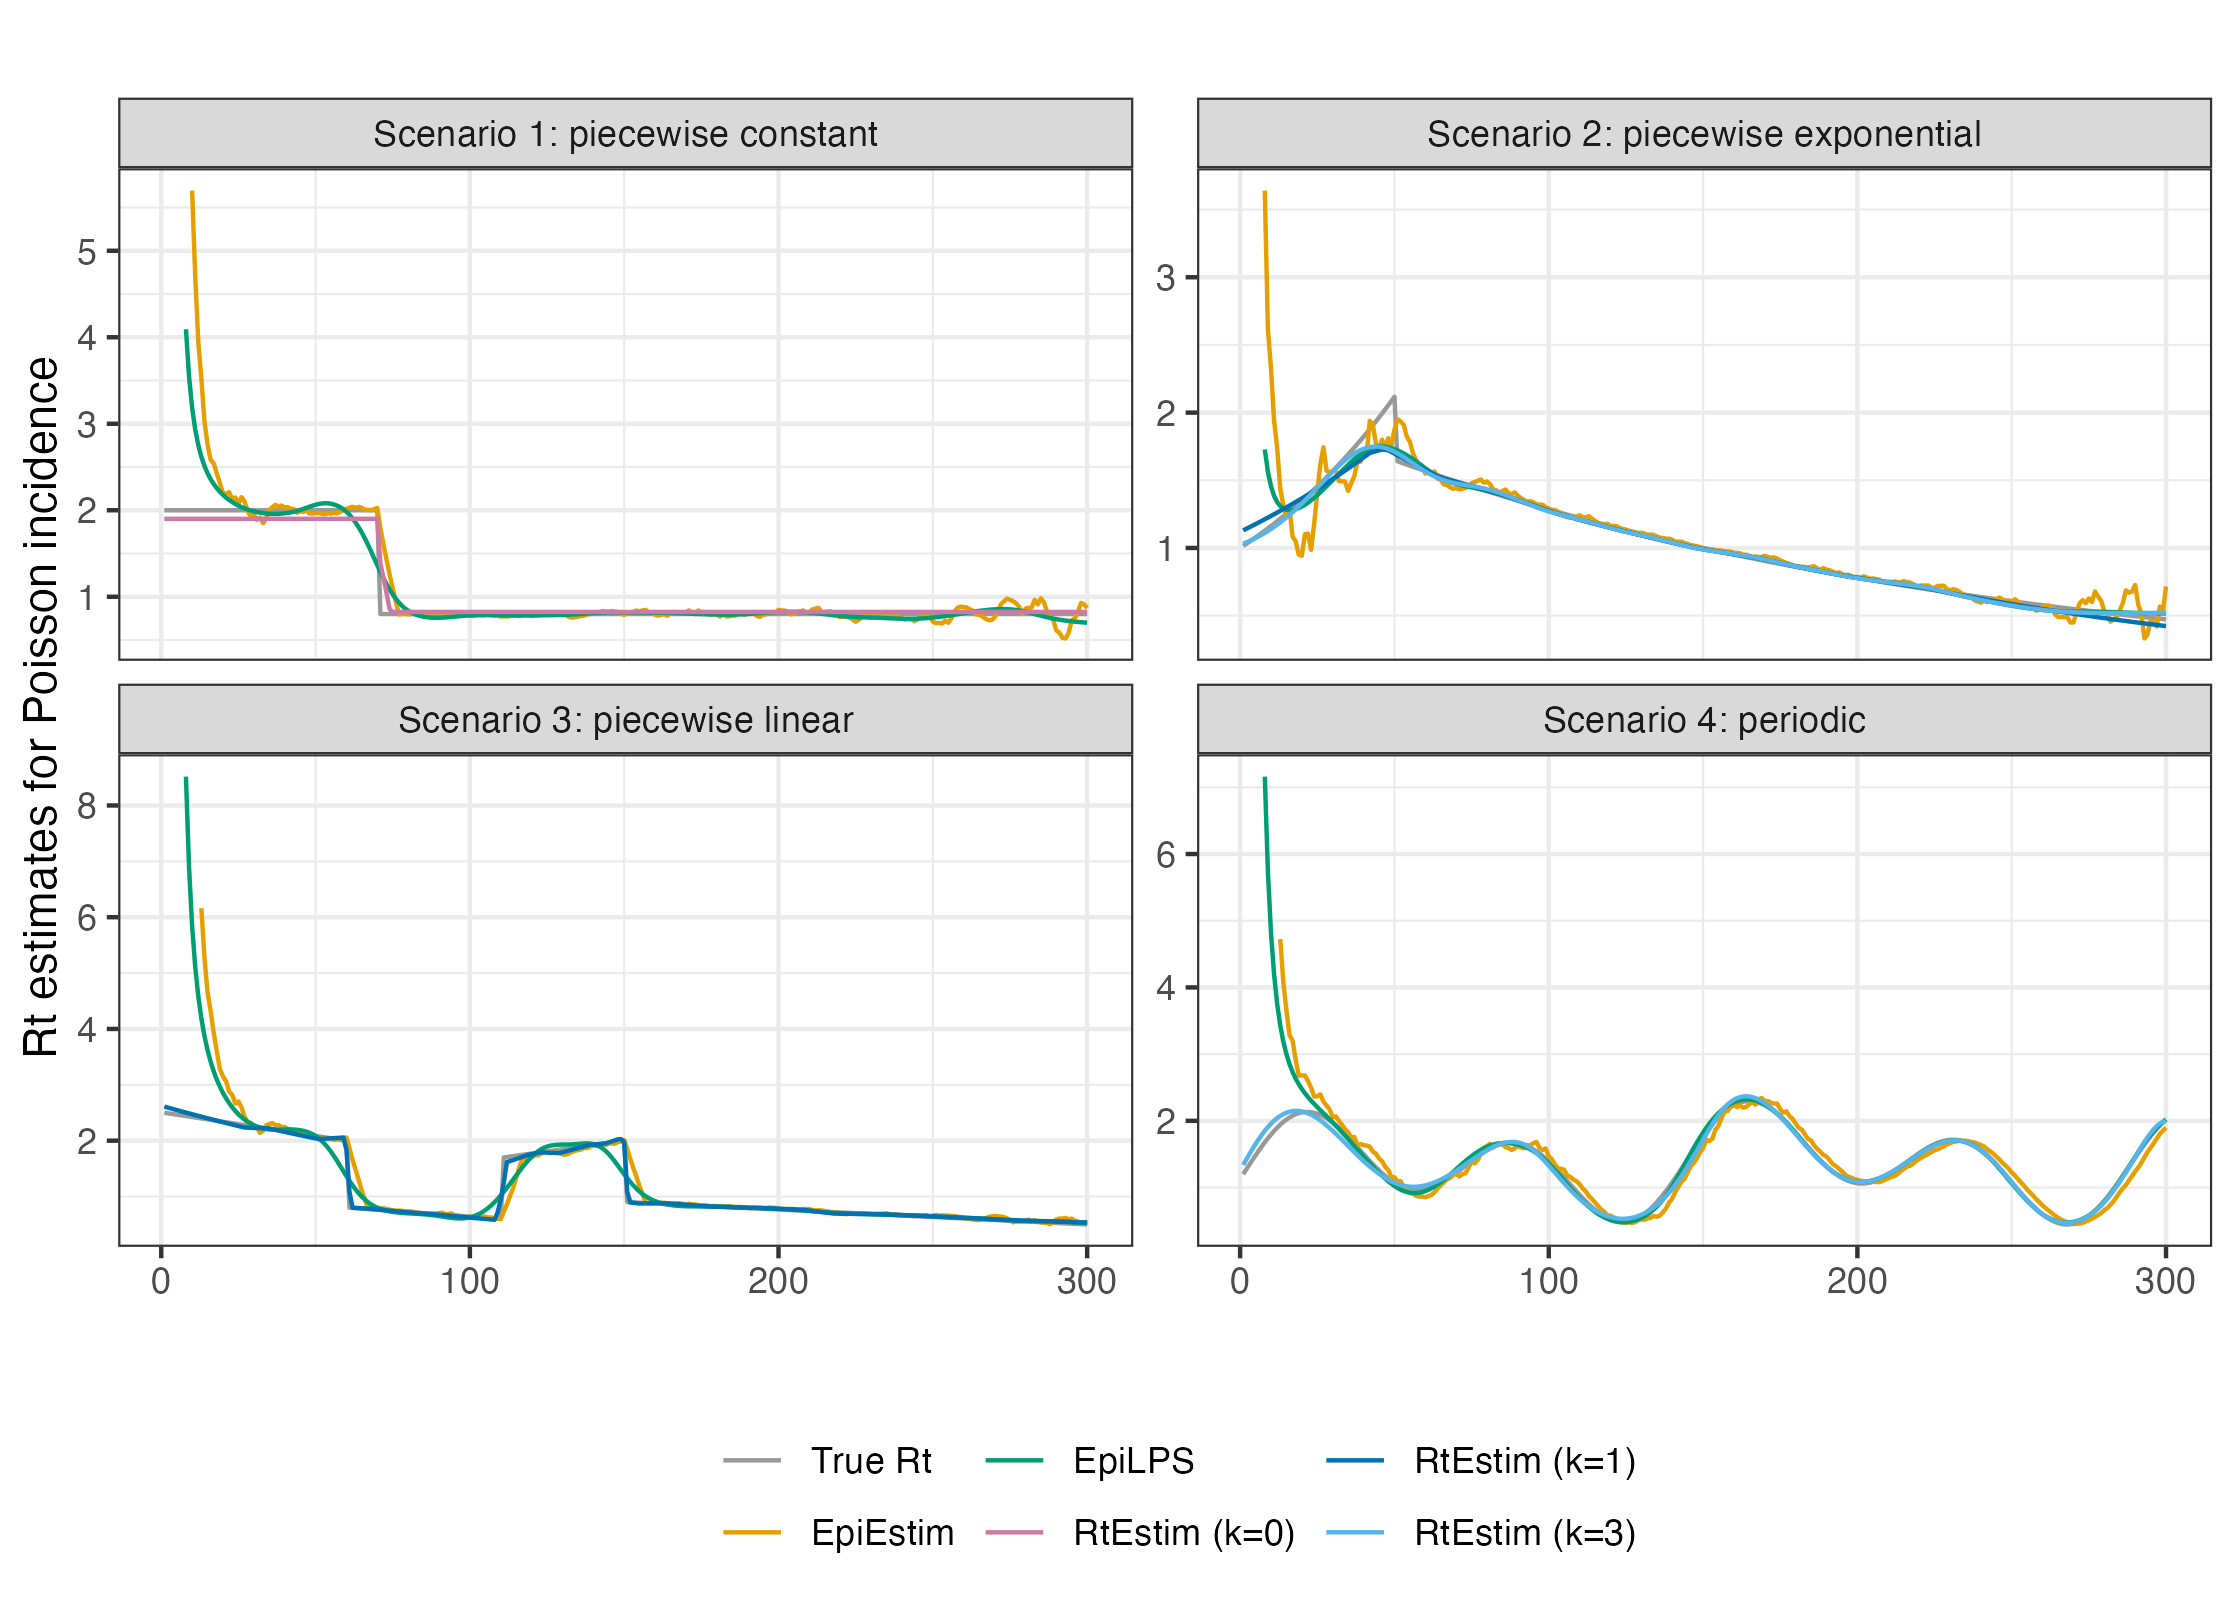
\includegraphics[width=.99\textwidth]{fig/Pois-res-plot.png}
    \caption{Example of effective reproduction number estimation for Poisson incidence.}
    \label{fig:pois-est}
\end{figure}


% experiment results under the violation of assumptions
To investigate the performance under the violation of the Poisson distributional
assumption (of both \RtEstim\ and \EpiEstim), we also examine estimation
accuracy with negative Binomial data. \autoref{fig:nb-est} displays a
realization, analogous to the previous case, for all methods and scenarios.
\RtEstim\ has more difficulty relative to the Poisson incidence setting,
especially at the beginning of the outbreak. This is most pronounced in Scenario
4, where \RtEstim\ is overly smooth, except in the last wave. In Scenario 2,
\RtEstim\ successfully captures the changepoint, but suffers from the same
problem as in the Poisson setting. In Scenario 3, the piecewise linear \RtEstim\
recovers the curvature of $\calR_t$ well, but is less accurate than
in the Poisson incidence.

\begin{figure}[tb]
    \centering
    \includegraphics*[width=.99\textwidth]{fig/NB-res-plot.png}
    \caption{Example of effective reproduction number estimation for negative Binomial
    incidence.}
    \label{fig:nb-est}
\end{figure}

Finally, it is important to provide a brief comparison of the running times of
three models across the $8$ experimental settings. We find that almost all
models across all experiments complete within $10$ seconds.
\RtEstim\ generally takes the longest, likely due to a relatively large
candidate set --- $50$ values of $\lambda$ and $10$ folds of cross validation --- while
other models run only a single time for a fixed setting of hyperparameters per
experiment. Additional results on timing comparisons are deferred to the
Appendix. 


\subsection{Real-data results: Covid-19 incident cases in British Columbia}

% introduce data & tuning parameter setup
We implement \RtEstim\ on Covid-19 incident confirmed cases in British Columbia
(B.C.) as reported on May 18, 2023 (visualized in \autoref{fig:covid-data}) by
the B.C.\ Centre for Disease Control. 
We use the gamma distribution with shape $2.5$ and scale $2.5$
to approximate the serial interval function, which is empirically
reasonable, since they are close to the parameters in a recent study 
\citep{lehtinen2021relationship}, which summarizes estimated parameters of the 
serial interval distributions of SARS-CoV-2 by different approaches. 

\begin{figure}[tb]
    \centering
    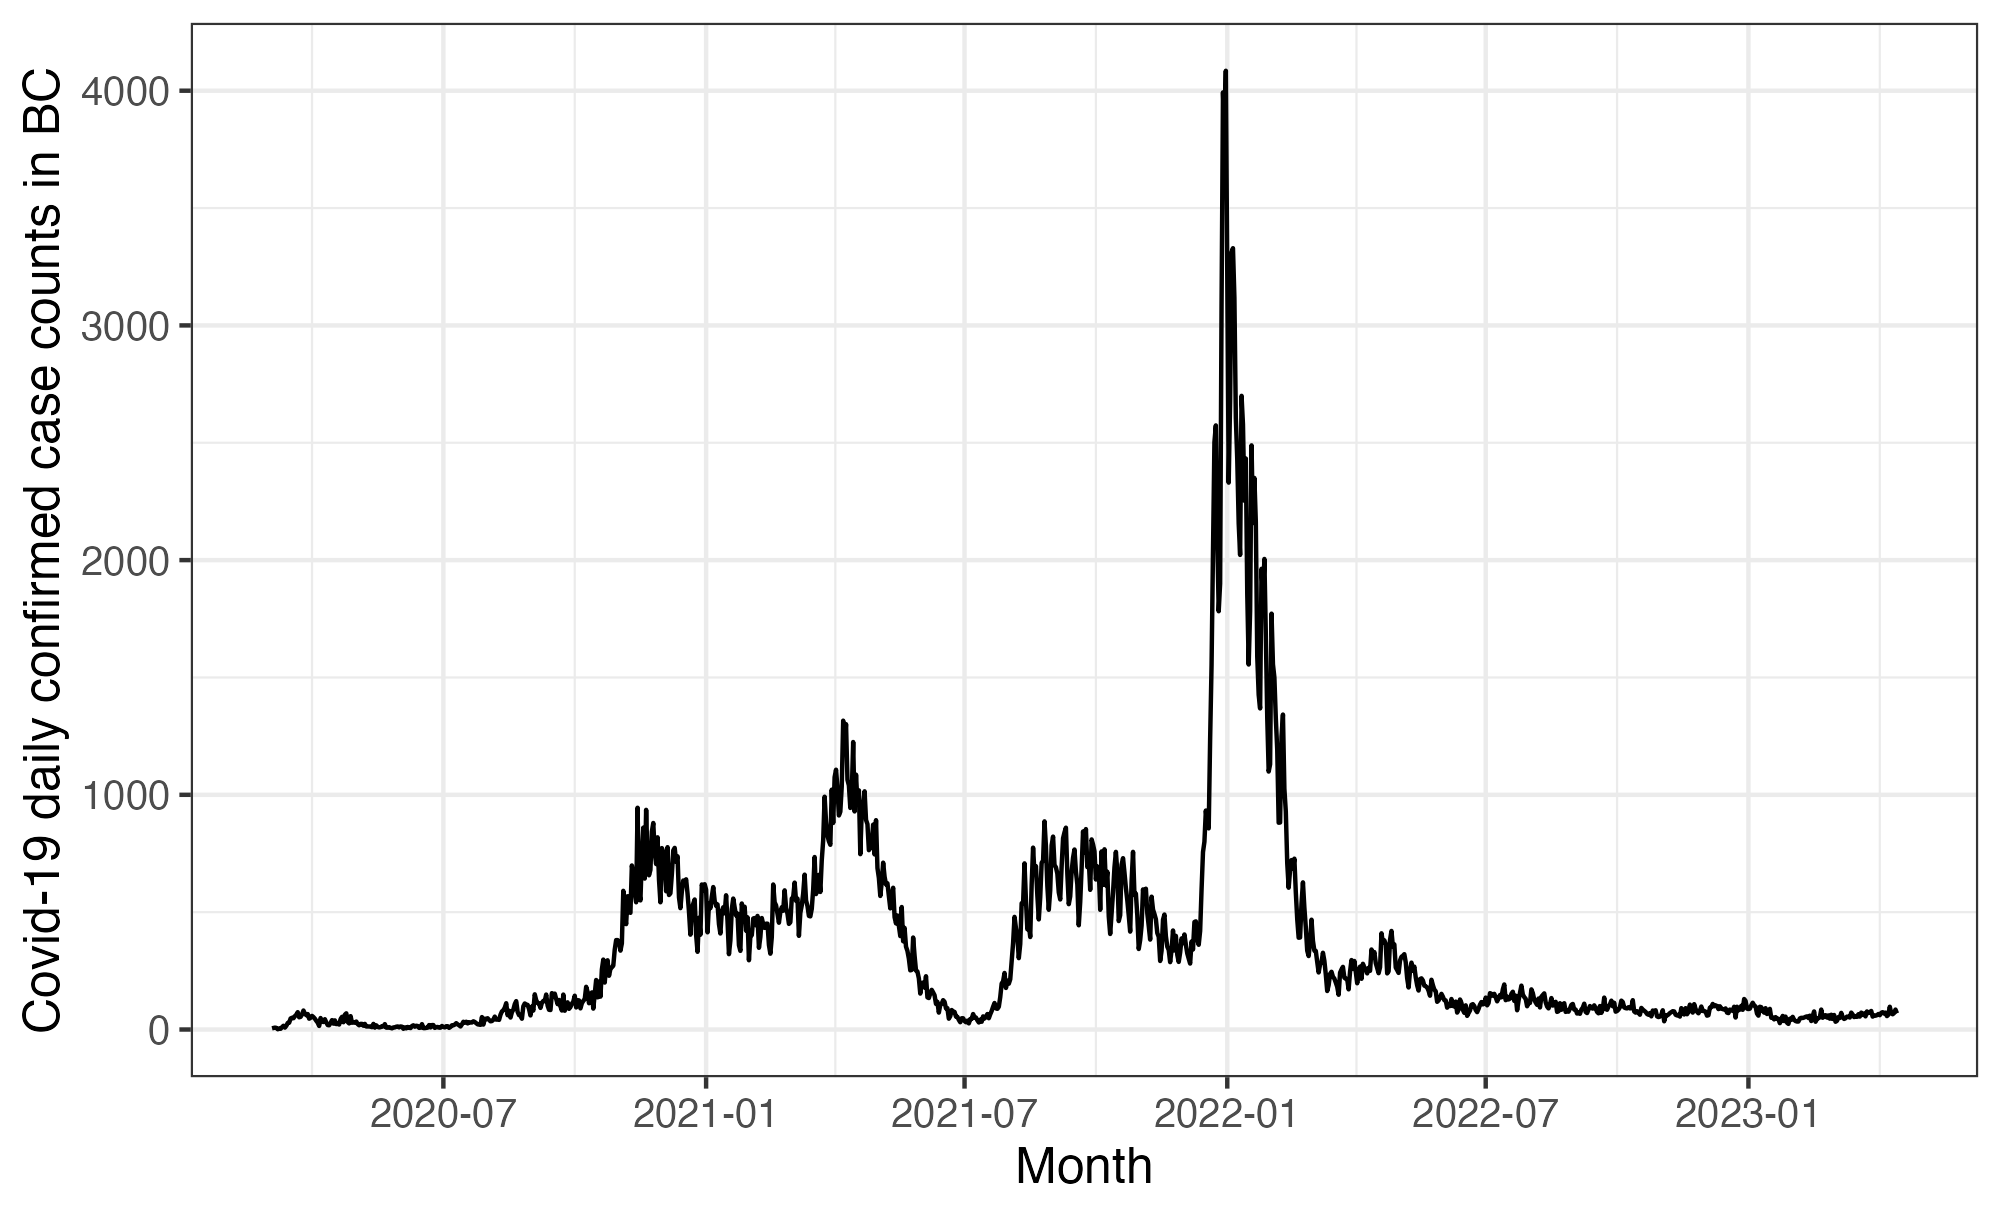
\includegraphics[width=0.9\textwidth]{fig/covid_dat.png}
    \caption{Covid-19 daily confirmed incident cases between March 1st, 
    2020 and April 15th, 2023 in British Columbia, Canada.} 
    \label{fig:covid-data}
\end{figure} 

% interpret figures -- across all lambdas
Considering the first, second, and third polynomial degrees, the estimated 
effective reproduction numbers of Covid-19 in British Columbia
(illustrated in \autoref{fig:covid-rt}) are always less than $3$ except at the 
very early stage, which means that one distinct infected individuals on average 
infects less than three other individuals in the population. 
Examining three different settings for $k$, 
the temporal evolution of $\widehat{\calR}$ (across all regularization levels
$\lambda$) are similar near the highest peak around the end of 2021 before
dropping shortly thereafter. Throughout the estimated curves, the peaks and
troughs of the reproduction numbers precede the growth and decay cycles of
confirmed cases, as expected. We also visualize 95\% confidence bands for the
point estimates at the smallest one of the ``optimal'' tuning parameters with 
lowest CV (i.e., KL divergence) scores in \autoref{fig:covid-rt}.     

The estimated reproduction numbers are relatively unstable before April 1st,
2022. The highest peak coincides with the emergence and global spread of the
Omicron variant. The estimated reproduction numbers fall below 1 during two time
periods --- roughly from April 1st, 2021 to July 1st, 2021 and from January 1st,
2022 to April 1st, 2022. The first trough coincides with the introduction of
Covid-19 vaccines in British Columbia. The second trough, shortly after the
greatest peak may be due to variety of factors resulting in the depletion of the
susceptible population such as increased self-isolation in response to the peak
and media and immunity incurred via recent infection. Since around April 1st,
2022, estimated reproduction numbers have remained relatively stable
(fluctuating around $1$) corresponding to low reported cases (though reporting
behaviours have also changed significantly since the Omicron wave). 

% for different lambda (DJM: not clear to me what the following adds. We should
% discuss the CV choice above.) Greater regularization levels (by using larger
% $\lambda$'s) result in smoother estimated curves. Smoother curves suggest that
% the estimated reproduction numbers are around $1$ during most time periods;
% however, it may miss to capture some outbreaks of the pandemic. More wiggly
% curves better reflect the fluctuation of $\calR_t$, but sometimes fail to
% highlight the significant peaks or troughs. The tuning parameter $\lambda$
% needs to be chosen corresponding to the information in practice for a better
% interpretation. Here, we provide the CV-chosen $\calR_t$ estimates with
% confidence bands. 

\begin{figure}[tb]
    \centering
    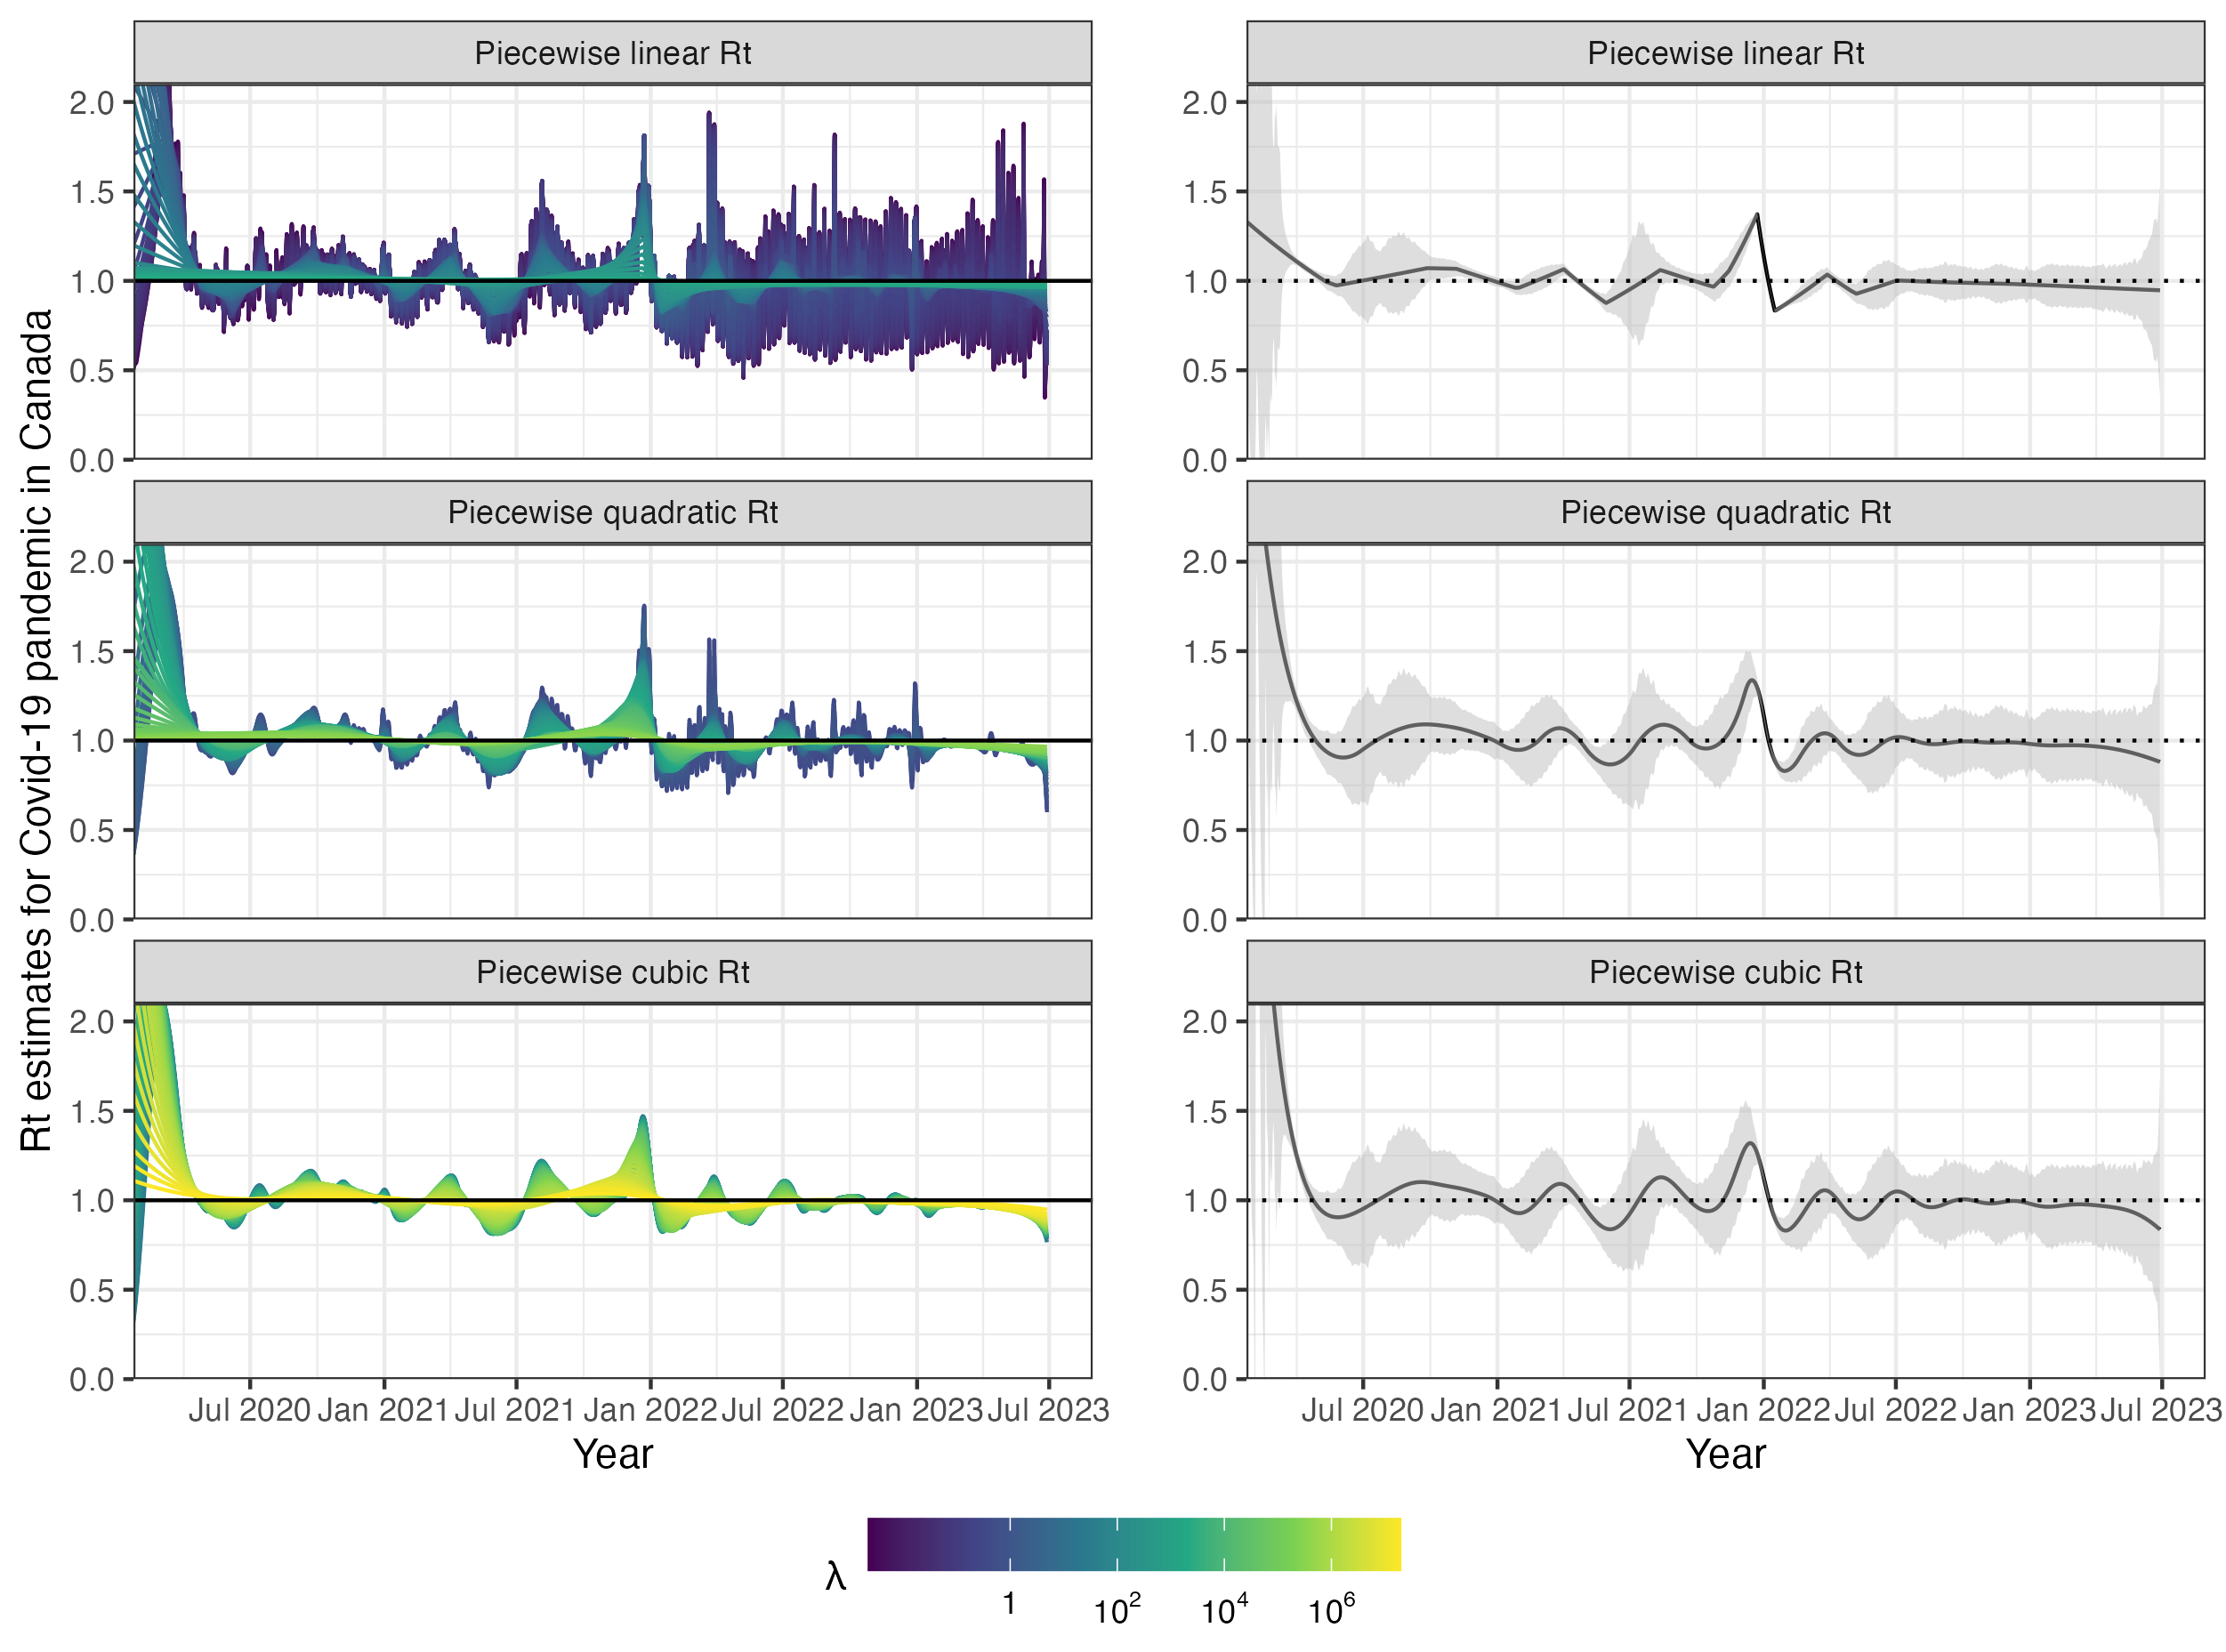
\includegraphics[width=0.9\linewidth]{fig/covid_full_res.png}
    \caption{Estimated effective reproduction numbers for Covid19 daily confirmed 
    counts between March 1st, 2020 and April 15th, 2023 in British Columbia, Canada. 
    The left panels demonstrate estimates corresponding to 50 tuning parameters. 
    The right panels display the CV-tuned estimates with 95\% confidence intervals. 
    The top, medium and bottom panels illustrate the estimated reproduction numbers 
    ($\calR_t$) using the Poisson trend filtering (in \eqref{eq:rt-ptf}) with 
    degrees $k=1,2,3$ respectively.} 
    \label{fig:covid-rt}
\end{figure} 


\subsection{Real-data results: Pandemic influenza in Baltimore, Maryland, 1918}

We also apply \RtEstim\ to daily reported influenza cases in Baltimore, Maryland
occurring during the world-wide pandemic of 1918 from September to November. 
The dataset (shown in \autoref{fig:flu-dat}) is included in the \EpiEstim\ \R\ package. 
The 1918 influenza outbreak, caused by the H1N1 influenza A virus, was unprecedentedly
deadly with case fatality rate over 2.5\%, infecting almost one-third of the population across the world
\citep{taubenberger20061918}. The CV-tuned piecewise cubic estimates in \autoref{fig:flu-res}
better capture the growth at the beginning of the pandemic in \autoref{fig:flu-dat}. 
The estimated $\calR_t$ curve suggests that the transmissibility of the pandemic 
grew rapidly over the first 30 days before declining below $1$ after 50 days. 
However, it also suggests an increase of the infectiousness toward the end of the period. 
With the currently available dataset, it is hard to tell if there is a next wave 
or a steady decline ahead. The CV-tuned piecewise 
constant and linear estimates in \autoref{fig:flu-res} both suggest a steady decline. 
This is supported by a couple of arguments. The influenza incidence reduces to $0$ in the end. 
The $\calR$ estimates of \EpiEstim\ with 1-week, 2-week and 4-week sliding windows 
in \cite{cori2013new} are all lower than the threshold $1$ in their right tails. 



\begin{figure}[tb]
    \centering
    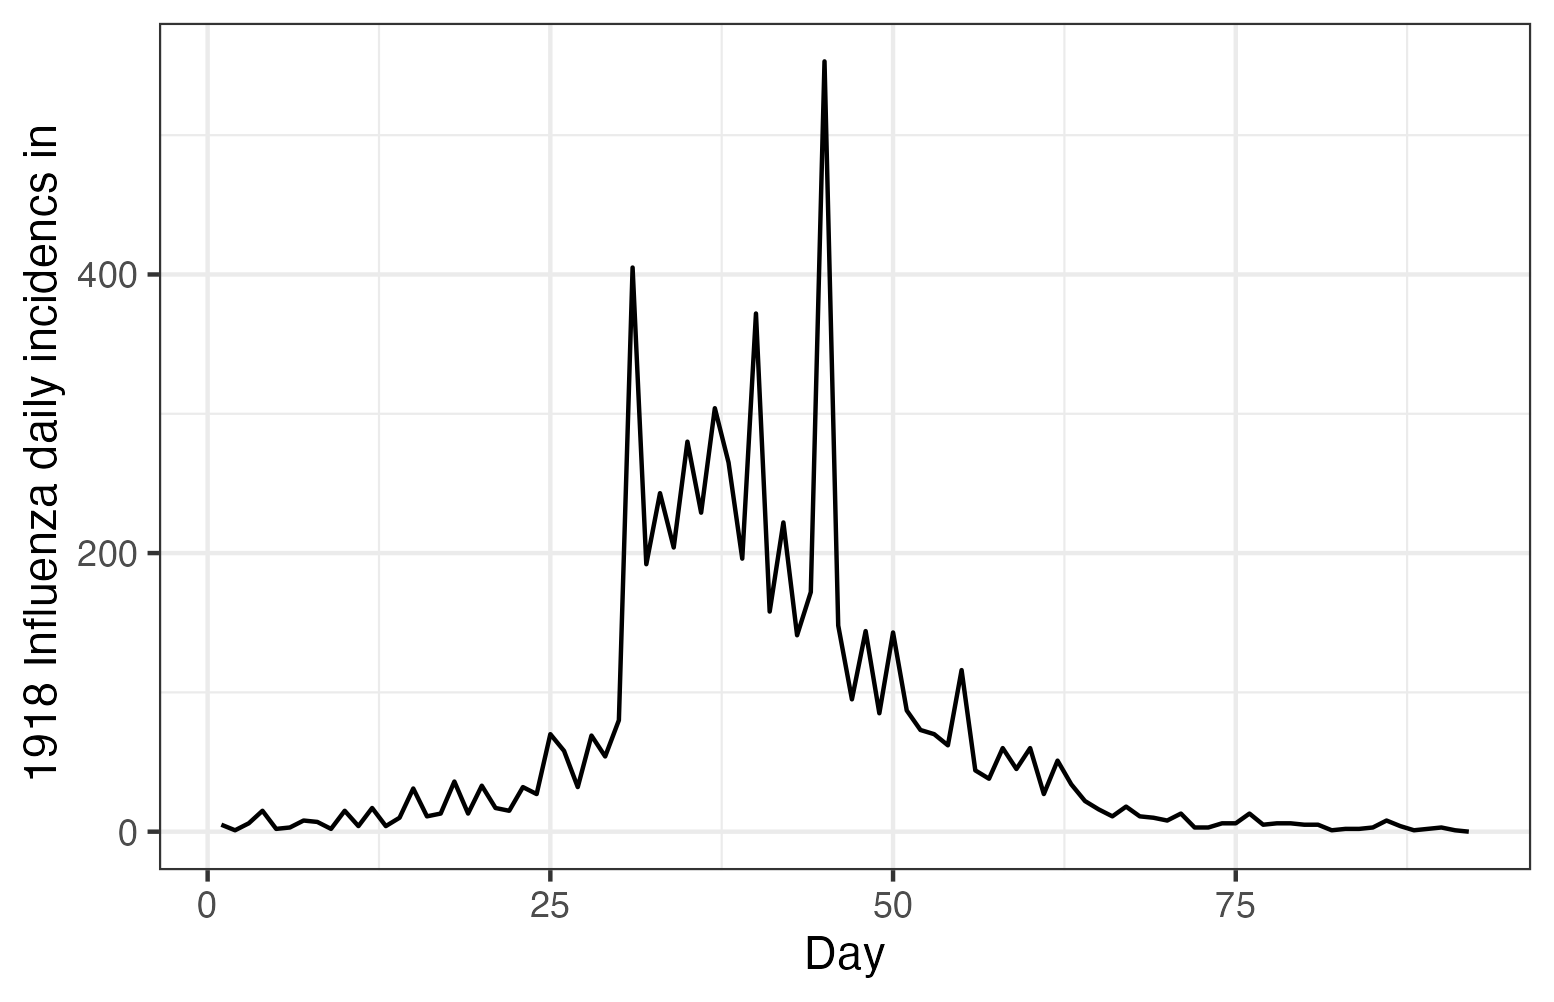
\includegraphics[width=0.9\linewidth]{fig/flu_dat.png}
    \caption{Daily influenza incident counts in Baltimore, Maryland between September 
    and November in 1918.} 
    \label{fig:flu-dat}
\end{figure} 

\begin{figure}[tb]
    \centering
    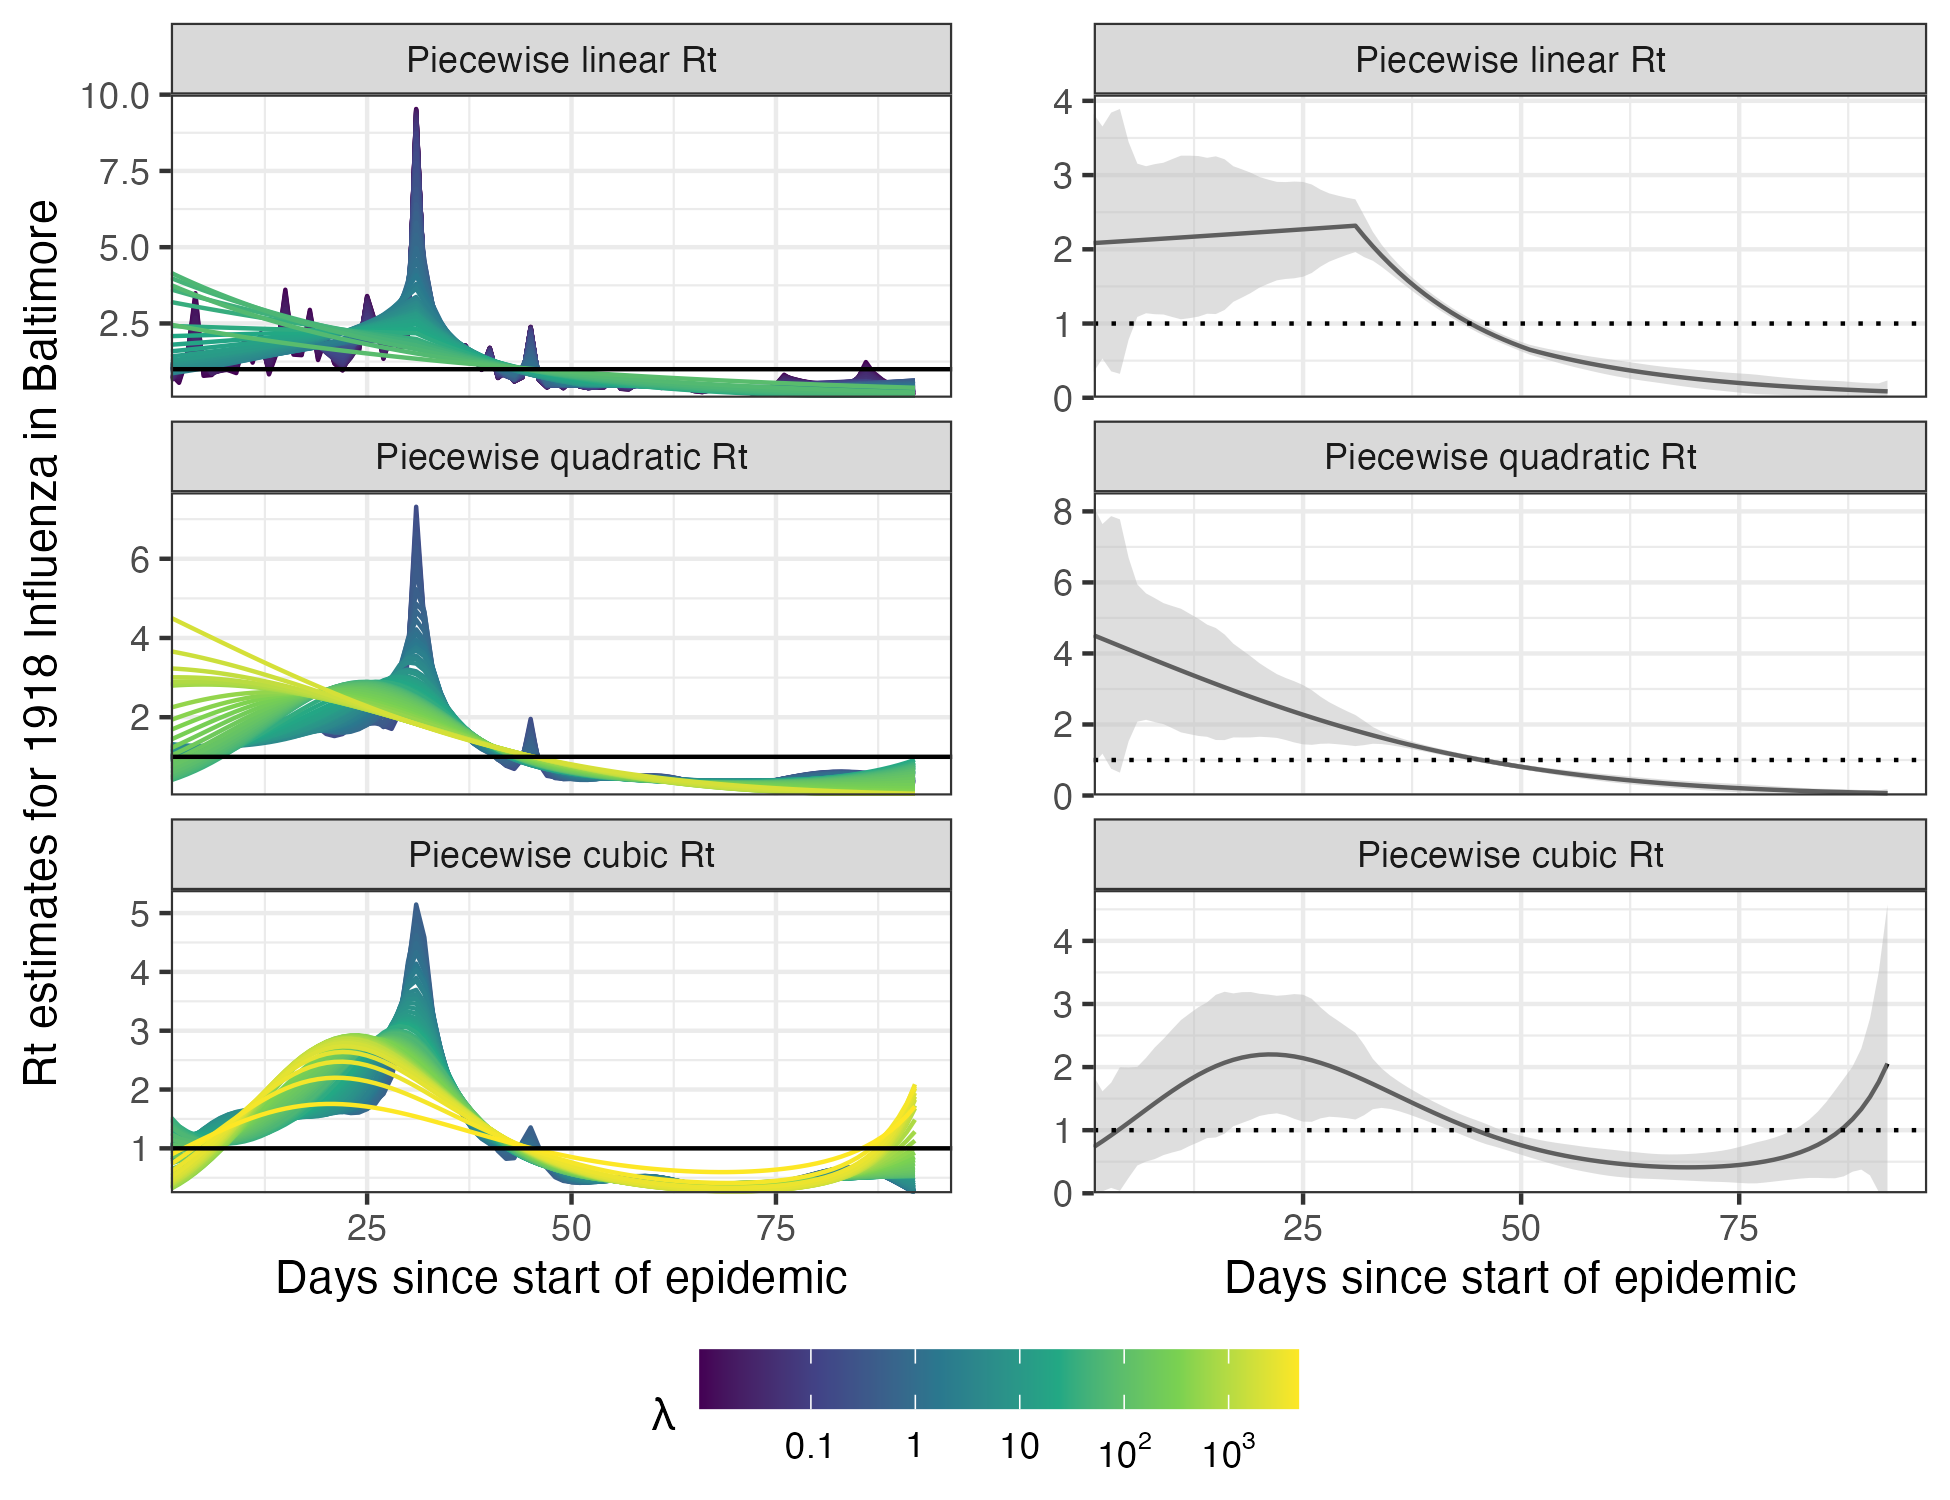
\includegraphics[width=0.9\linewidth]{fig/flu_full_res.png}
    \caption{Estimated effective reproduction numbers for influenza in
    Baltimore, Maryland in 1918. The left panels show estimates for all
    50 tuning parameters under consideration. The right column displays the 
    CV-tuned estimates with 95\% confidence bands. The rows (top to bottom) show
    estimated reproduction numbers ($\calR_t$) using the Poisson trend filtering
    (in \eqref{eq:rt-ptf}) with degrees $k=1,2,3$ respectively.} 
    \label{fig:flu-res}
\end{figure} 

